\chapter{Methoden}
\section{nnU-Net}
\subsection{Allgemein}
nnU-Net von \citeauthor{Isensee.2021} steht für \glqq no new (U-)Net\grqq{} und ist ein Framework zur Segmentierung von medizinischen Bildern basierend auf der U-Net-Architektur. Das besondere an nnU-Net ist, dass es nur mit einem Set von drei U-Net-Modellen mit kleinen Änderungen zum original U-Net-Modell arbeitet. Es wurde speziell dafür Entworfen auf nahezu allen medizinischen Datensätzen zu funktionieren ohne es für einen bestimmten Anwendungsfall anzupassen. nnU-Net konfiguriert sich automatisiert selbst durch Adaption am Datensatz und konzentriert sich dabei auf Schritte bei denen viel Performanz gewonnen werden kann, wie:
\begin{itemize}
\item Preprocessing (z.B. Resampling und Normalisierung)
\item Training (z.B. Loss- und Optimizereinstellungen sowie Data-Augmentation)
\item Inferenz (z.B. Patch basierte Strategie und Ensembling)
\item Post-Processing (z.B. erzwingen von Single-Connected Components)
\end{itemize}

Wie in Abbildung \ref{fig:nnUNetConfig} zu sehen ist basiert die automatische Konfiguration auf drei Parametergruppen: fixierte, regelbasierte und empirische Parameter. Dabei werden zuerst die festen Parameter gesammelt und optimiert. Im zweiten Schritt werden die regelbasierten Parameter ermittelt. Hierfür werden Metadaten des Datensatzes, wie Bildgröße und Modalität, herangezogen aber auch andere Faktoren wie der verfügbare GPU-Speicher werden beachtet. Anhand dieser Daten werden die drei U-Net-Modelle trainiert. Im dritten Schritt werden die Trainingsdaten ausgewertet und abhängig davon wird das Modell sowie die Post-Processing-Routine festgelegt. Die Art und Weise wie nnU-Net arbeitet wurde an zehn verschiedenen Datensätzen der Medical Decathlon Segmentation Challenge getestet und erreichte den höchsten Dice-Score für alle Klassen, außer Klasse 1 BrainTumour, der Phase 1 Aufgaben. (\cite{Isensee.2018})

\begin{figure}[H]
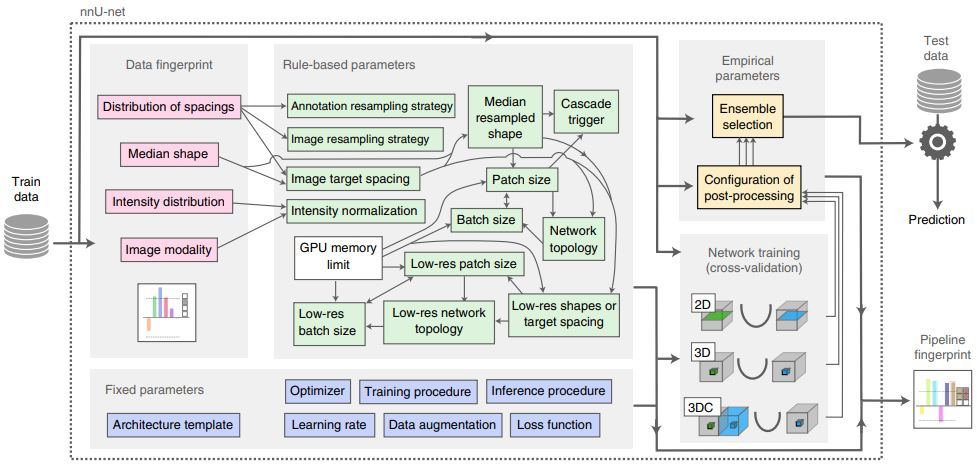
\includegraphics[width=\linewidth]{./images/nnUnetAutomatedMethodConfig.jpg}
\captionof{figure}{nnU-Net automatisierte Konfiguration Quelle: \cite[S. 3]{Isensee.2021}}
\label{fig:nnUNetConfig}
\end{figure}


\subsection{Anwendung}
Im Folgenden gehe ich nun auf die Anwendung von nnU-Net in der Studienarbeit ein. Um die Arbeitsschritte besser nachvollziehen zu können wurden diese in einem Jupyter Notebook zusammengefasst. Dieses wurde auf Basis des nnU-Net Workshops von \cite{Luth.2022} erstellt. In diesem wurden folgende Arbeitsschritte durchgeführt:
\begin{itemize}
\item Aufsetzen der nnU-Net Ordnerstruktur und setzen der benötigten Umgebungsvariablen
\item Datenvorbereitung (Entpacken und vorbereiten der dataset.json-Datei)
\item Datensatzkonvertierung mithilfe von nnU-Net
\item Vorbereitung des Trainings via nnU-Net
\item Training mit nnU-Net
\item Inference mit nnU-Net
\item Visualisierung der Ergebnisse
\item Auswertung der Ergebnisse
\end{itemize}

Da für die Verwendung von nnU-Net eine gewisse Ordnerstruktur benötigt wird, wird diese zu Beginn erstellt. Zusätzlich werden für die Pfade dieser, die von nnU-Net benötigten, Umgebungsvariablen gesetzt. Der bereits hinterlegte Datensatz wird entpackt und die benötigte dataset.json-Datei wird, wie in Abschnitt \ref{Usage} beschrieben, vorbereitet.

Die dann folgenden Arbeitsschritte wurden mithilfe von nnU-Net durchgeführt. Der Datensatz wird durch den Aufruf
\begin{lstlisting}
nnUNet_convert_decathlon_task -i PATH_TO_RAWDATA_FOLDER
\end{lstlisting}
so konvertiert, dass dieser für nnU-Net nutzbar ist.
Der Parameter \newline \glqq PATH\char`_TO\char`_RAWDATA\char`_FOLDER\grqq{} gibt dabei den Pfad zum Verzeichnis der Rohdaten an. 

Durch
\begin{lstlisting}
nnUNet_plan_and_preprocess -t TASK_NAME_OR_ID
\end{lstlisting}
wird der Datensatz analysiert und die regelbasierten Parameter ermittelt. \newline \glqq PATH\char`_TO\char`_RAWDATA\char`_FOLDER\grqq{} spezifiziert dabei die Tasknummer welche über den Verzeichnisnamen festgelegt wird.

Durch 
\begin{lstlisting}
nnUNet_train \
	CONFIGURATION \
	TRAINER_CLASS_NAME \
	TASK_NAME_OR_ID \
	FOLD\
	/
\end{lstlisting}
wird das Training gestartet. In dieser Arbeit erfolgte der Aufruf
\begin{lstlisting}
nnUNet_train 3d_fullres nnUNetTrainerV2 1 0
\end{lstlisting}
wodurch das Training mit der \glqq 3D-Full-Resolution\grqq{} Konfiguration und der Trainerklasse \glqq nnUNetTrainerV2\grqq{} für die Task-ID \glqq 1\grqq{} gestartet wurde.

Für die gewählte Trainerklasse erfolgte nun ein Training für 1000 Epochen wobei dieses nach 239 Epochen, aus zeitlichen Gründen, händisch unterbrochen wurde. Alternativ hätte eine eigene Trainerklasse erstellt werden können, die eine geringere Anzahl von Epochen trainiert hätte. Auf diesen Hinweis bin ich jedoch erst später gestoßen und da das Unterbrechen keine Auswirkung auf das resultierende Modell hat wurde dies nicht weiterverfolgt. Aufgrund der Unterbrechung mussten jedoch die gespeicherten Modelle umbenannt werden (siehe Jupyter Notebook). 

Im nächsten Schritt erfolgt bereits die Verwendung des trainierten Modells. Durch
\begin{lstlisting}
nnUNet_predict \
	-i INPUT_PATH \
	-o OUTPUT_PATH \
	-t TASK_NAME_OR_ID \
	-tr TRAINER_CLASS_NAME \
	/
\end{lstlisting}
können nun die gewünschten Label für die Eingabebilder vorhergesagt werden.

Mit dem Befehl 
\begin{lstlisting}
nnUNet_evaluate_folder \
	-ref LABELS_PATH \
	-pred PREDICTIONS_PATH \
	-l LABEL_INDEX1 LABEL_INDEX2 ... \
	/
\end{lstlisting}
können die ermittelten Labels durch einen Vergleich mit den den originalen Labels evaluiert werden.

\section{Monai SegResNet}
\subsection{Allgemein}
SegResNet von \cite{Myronenko.2018} ist ein Segmentierungsansatz der auf einer Encoder-Decoder basierten CNN-Architektur aufsetzt.

\begin{figure}[H]
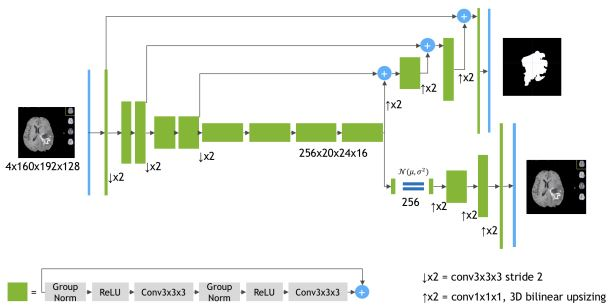
\includegraphics[width=\linewidth]{./images/SegResNet.jpg}
\captionof{figure}{Schematische Visualiserung der Netzwerkarchitektur von SegResNet Quelle: \cite[S. 3]{Myronenko.2018}}
\label{fig:SegResNet}
\end{figure}

In Abbildung \ref{fig:SegResNet} sieht man eine schematische Visualisierung der Architektur. Die Eingabe ist ein Vier-Kanal 3D MRT Bild gefolgt von einer 3x3x3 3D Convolution mit 32 Filtern. Die grünen Blöcke stellen ResNet-ähnliche Blöcke mit GroupNorm normalisierung dar. Im Originalpaper von \cite{Myronenko.2018} wurde das Bild zunehmend um zwei Dimensionen verkleinert und die Anzahl der Features um zwei erhöht. Der Decoder-Teil ist ähnlich dem Encoder, jedoch mit einem Block pro Dimension. Jede Decoderstufe beginnt mit einer Vergrößerung, welche die Anzahl der Features halbiert (durch 1x1x1 Convolutions) und mithilfe von 3D bilinear upsampling die Anzahl der Dimensionen verdoppelt, gefolgt von einer Addition der Encoder-Outputs derselben räumlichen Ebene. Die Ausgabe des Segmentierungsdecoder hat dieselbe Größe wie das ursprüngliche Bild und dieselbe Anzahl an Features wie die Eingabe. Durch eine weitere 1x1x1 Convolution wird das Bild in drei Kanäle transformiert gefolgt von einer Sigmoid-Funktion. Der VAE (variational auto-encoder)-Branch rekonstruiert das Eingabebild und wird nur während des Trainings zur Regularisierung des Encoders benutzt. Grund für die Nutzung des Auto-Encoder-Branches ist die limitierte Verfügbarkeit der Daten.

\subsection{Anwendung}
Im Folgenden gehe ich auf die Anwendung des SegResNet in der Studienarbeit ein. Dafür wurde ein Jupyter Notebook erstellt, das alle Arbeitsschritte zusammenfasst. Jedoch verwende ich nicht die ursprüngliche Implementierung von \cite{Myronenko.2018}, sondern die Implementierung des Monai-Frameworks. Dabei wurde zur Hilfe das \citetitle{Monai.2020}-Tutorial von Monai verwendet.

\subsubsection{Dataloader}
Die benötigten Daten wurden mithilfe der Monai CacheDataset-Klasse und der DataLoader-Klasse geladen. Die CacheDataset-Klasse besitzt einen Cache-Mechanismus der Daten lädt und deterministische Datentransformationen darauf cached. Daraus resultiert ein deutlich schnelleres Laden der Daten beim Training. 

\begin{figure}[H]
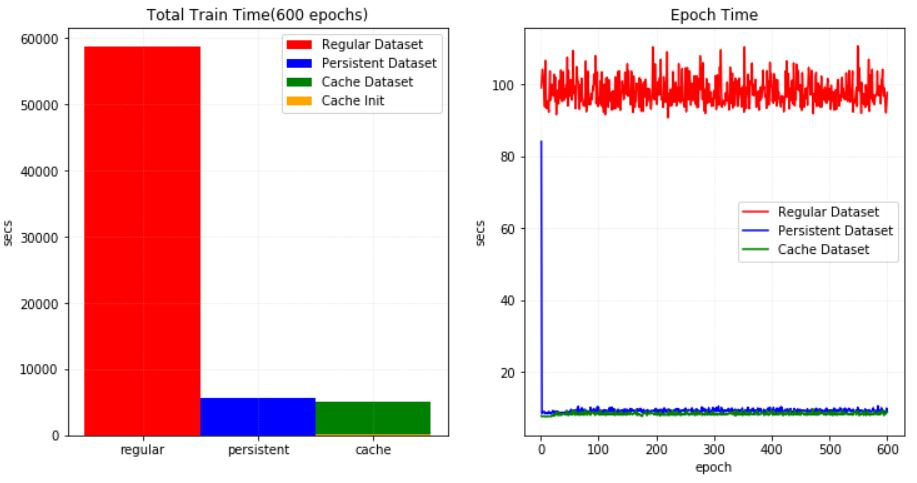
\includegraphics[width=\linewidth]{./images/cachedataset.jpg}
\captionof{figure}{Visualisierung der Trainingsgeschwindigkeit mit verschiedenen Dataloadern Quelle: \cite{Dataloader.2020}}
\label{fig:dataloader}
\end{figure}

\subsubsection{Transforms}
Bei der Datenaugmentierung wird zuerst sichergestellt, dass beim Bild der Channel an erster Stelle steht. Dies gewährleistet die Funktion EnsureChannelFirstd. Danach werden die Labels in 3 Kanäle aufgeteilt. Durch die Orientationd-Funktion werden Bild und Label in ein normalisiertes Koordinatensystem transformiert. Daraufhin werden beide, durch Spacingsd, in dieselbe Pixeldimension gebracht. Danach wird ein 224x244x144 Bereich des Bildes mit zufälligem Mittelpunkt ausgeschnitten. Da die wichtigen Bereiche des Bildes im Zentrum liegen und das Bild vor dem zuschneiden eine Form von 240x240x155 hat, gehen keine wichtigen Elemente des Bildes verloren und dennoch unterscheidet sich das Bild jedes Mal vom Original. Abbildung \ref{fig:crop} zeigt das Ergebnis des Zuschneidens. Zu beachten ist, dass das Zuschneiden auch auf der Z-Achse geschieht und dadurch diese nicht in beiden Bildern gleich ist.

\begin{figure}
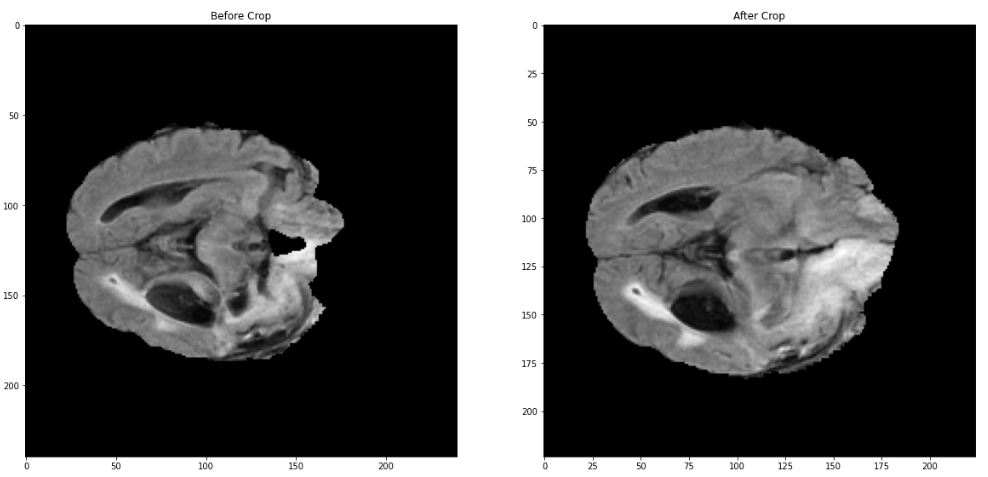
\includegraphics[width=\linewidth]{./images/Crop.jpg}
\captionof{figure}{Bild vor und nach dem RandSpatialCrop}
\label{fig:crop}
\end{figure}

Nach dem RandSpatialCropd erfolgt ein zufälliger Flip, durch RandFlipd, auf jeder Achse. Der Zufall besteht hierbei darin, dass der Flip zu 50\% durchgeführt wird.

\begin{figure}[H]
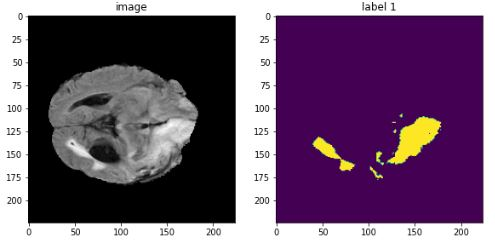
\includegraphics[width=\linewidth]{./images/beforeFlip.jpg}
\captionof{figure}{Bild und Label 1 vor dem Flip}
\label{fig:beforeFlip}
\end{figure}

In den Abbildungen \ref{fig:flip1}, \ref{fig:flip2}, \ref{fig:flip3} sieht man die Ergebnisse jedes Flips, wenn dieser durchgeführt wird.

\begin{figure}[H]
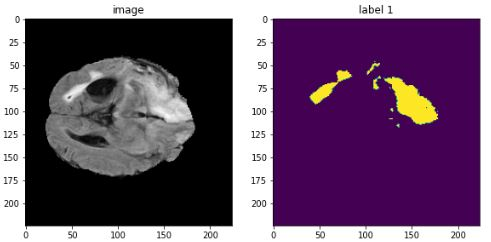
\includegraphics[width=\linewidth]{./images/flipAxis0.jpg}
\captionof{figure}{Bild und Label 1 nach dem Flip auf Achse 0}
\label{fig:flip1}

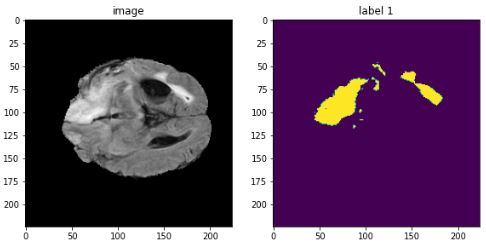
\includegraphics[width=\linewidth]{./images/flipAxis1.jpg}
\captionof{figure}{Bild und Label 1 nach dem Flip auf Achse 1}
\label{fig:flip2}
\end{figure}

In den letzten drei Schritten wird die Intensität des Bildes transformiert. Zuerst wird die Intensität durch NormalizeIntensity normalisiert. Danach wird die Intensität zufällig skaliert und im letzten Schritt um einen zufälligen Offset verschoben. In Abbildung \ref{fig:intensity} sieht man die Auswirkung der Normalisierung gut. Die zufälligen Transformationen sind mit dem bloßen Auge jedoch kaum zu erkennen.

\begin{figure}[H]
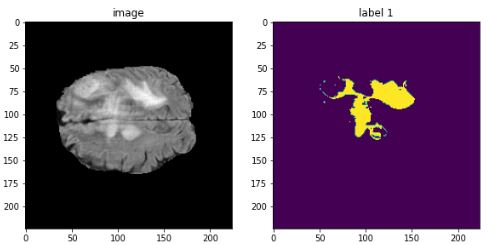
\includegraphics[width=\linewidth]{./images/flipAxis2.jpg}
\captionof{figure}{Bild und Label 1 nach dem Flip auf Achse 2}
\label{fig:flip3}
\end{figure}

\begin{figure}[H]
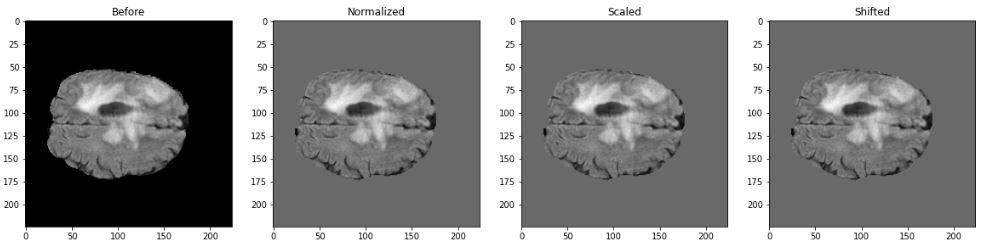
\includegraphics[width=\linewidth]{./images/intensityTransforms.jpg}
\captionof{figure}{Intensitätstransformationen}
\label{fig:intensity}
\end{figure}


\subsubsection{Training}
Zum Training wurde ein SegResNet mit den Parametern
\begin{itemize}
\item blocks\_down=[1,2,2,4]
\item blocks\_up=[1,1,1]
\item init\_filters=16
\item in\_channels=4
\item out\_channels=3
\item dropout\_prob=0.2
\end{itemize}
initialisiert. Die Blocks UP und Down entsprechen dabei dem Schema aus Abbildung \ref{fig:SegResNet}. Die initialen Filter geben dabei die Anzahl der Ausgabekanäle des initialen Convolutionlayers an. Die Eingabekanäle entsprechen hier den 4 Eingabebildern, also den 4 Modalitäten des 3D-Bildes. Die Ausgabekanäle entsprechen hierbei den drei Labels. Dropout\_prob gibt hierbei an, mit welcher Wahrscheinlichkeit ein Element genulled wird. Dies ist eine Methode zur Regularisierung und soll Overfitting vermeiden. Als Loss-Funktion wird der Dice-Loss verwendet sowie Adam als Optimizer. Danach wird das Training mit einer Batchsize von zwei gestartet. Im Training wird für jede Epoche der durchschnittliche Loss sowie der Dice-Score jedes Labels des Validierungsdatensatzes gespeichert. Sofern das Modell einen besseren Dice-Score erreicht, wird das Modell zwischengespeichert. Wie bei nnU-Net wurde wieder mit 239 Epochen trainiert um im nächsten Kapitel die beiden miteinander vergleichen zu können.
